\chapter{Conclusion}\label{ch:conclusion}

In conclusion, a thorough analysis of the literature and of the Namuru receiver has been developed. Additionally, Laplace domain modelling of the current implementation has been carried out, and a software model is currently being actively developed, to allow for more sophisticated modelling of the receiver. 


In order to achieve the goals of this thesis, a significant quantity of further work is required. 

Tasks include : 
\begin{itemize}
\item{Extending the software model to take into account jitter and lags}
\item{Extending the software model to take into account the effect of dynamics on the crystal}
\item{Validate the model against the existing receiver}
\item{Use a Monte Carlo simulation of the receiver to perform a parametric study of the receiver}
\item{Implementation of an improved algorithm on the Namuru Receiver}
\end{itemize}

The advantages of a parametric study using a Monte Carlo simulation of the receiver is that the incredibly complex behavior and nonidealities of the receiver can be accounted for. Additionally, development of a soft receiver allows new algorithms to be rapidly implemented in python, rather than in embedded C, allowing new ideas to be effectively evaluated. 

Validation of the receiver against the model is another important step. In order for the software model to be used to predict the behavior of the Nauru receiver, we must first be confident that it has the same behavior. The most effective way to evaluate if the model is accurate, is to determine if the model looses phase lock, at the same point during testing as the Namuru receiver. 

Understanding the dynamics of the crystal is also important, as vibrations during launch, and jerk during stage separation can lead to shifts in the \ac{LO} frequency. Hence the crystal in the Namuru receiver must be tested for sensitivity to acceleration. The most effective way to carry this out, is to conduct a "2g tip-over test", where the \ac{LO} frequency is measured, and the board is turned 180 degrees, and the \ac{LO} frequency is measured again. The change in frequency is divided by 2, to find the shift in Hz per g of acceleration. 

The development of software, by its nature is vulnerable to over-runs, so a careful plan, with generous timing has been developed, based on progress made in Thesis A. The plan for Thesis B can be seen in figure \ref{fig:ThesisBGantt}.

\begin{figure}[!htb] 
    \centering
    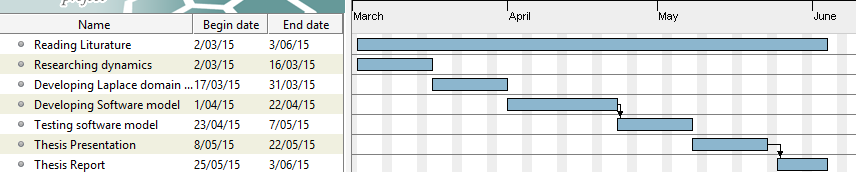
\includegraphics[width=1\textwidth]{ThesisPlanA.png} 
    \caption{Thesis A Gantt Chart}
    \label{fig:ThesisAGantt}
\end{figure}

\begin{figure}[!htb] 
    \centering
    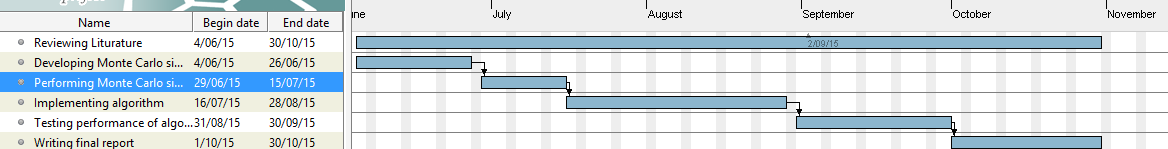
\includegraphics[width=1\textwidth]{ThesisPlanB.png} 
    \caption{Thesis B Gantt Chart}
    \label{fig:ThesisBGantt}
\end{figure}

The goals of this thesis can be quantified by evaluating the improvements to the performance of the Namuru receiver, by evaluating its performance using a \ac{GNSS} simulator. By using an accurate model of a \ac{SV} launch developed by Dr Eamonn Glennon, the performance can be evaluated under realistic conditions.




